\chapter{Theoretische Grundlagen}
\label{chap:two}
In diesem Kapitel wird der theoretische Rahmen für die weiteren Kapitel gelegt. Im
ersten Abschnitt werden die Grundlagen der Budgetplanung und Mittelallokation im Zusammenhang mit bibliothekarischen Statistiken erläutert. 
Der darauffolgende Abschnitt handelt von Datenvisualisierungen und deren Einsatz
für Datenrepräsentationen und Datenpräsentation. Abschließend wird das Modell der \textit{\acrlong{BI}-Systeme} als dritter Baustein zur Lösung der 
Problemstellung dieser Arbeit vorgestellt.

\section{Bibliothek und Statistik}
\label{chap:two_one}
% Bibliotheksrahmen - Etatplanung - Etatbedarfe, Zielsetzung der Bibliothek
Die Etatplanung von Bibliotheken richtet sich nach deren Informations- und Versorgungsauftrag. 
Seit Beginn der 1990er Jahre müssen sich Bibliotheken mit den Auswirkungen einer veränderten Medienlandschaft auseinandersetzen.
Sie kämpfen mit einem größer werdenden Informationsangebot, den steigenden Preisen auf dem Publikationsmarkt, 
den zunehmenden Kommerzialisierungstendenzen in der Verlagslandschaft und neuen Medientypen. 
Zu nennen wären hier konkret: die Explosion der Zeitschriftenpreise im Bereich der \acrfull{STM}, die Konzentration auf wenige Verlage, 
und dem Aufkommen von ebooks. Demgegenüber steigen Bibliotheksetats nur mäßig. 
Demzufolge geht ein Kaufkraftverlust der Bibliotheken einher \cite[vgl.][164 ff.]{moravetz-kuhlmann_monika_erwerbungspolitik_2015}.
%Diese Entwicklung betrifft nicht nur Universitätsbibliotheken, sondern auch Spezialbibliotheken von Forschungseinrichtungen.
Bibliotheken haben gegen diesen Trend Instrumente entwickelt, um den Informationsauftrag trotz dieser Widrigkeiten zu erfüllen.
So entstehen seit Mitte der 1990er Jahre von Bund und Ländern geförderte Konsortien, um den Kostendruck auf Bibliotheken insbesondere im Bereich der elektronischen
Fachinformationen zu mildern. Neue Geschäftsmodelle werden zur Abfederung der Kosten entwickelt, um Preisnachlässe bei großen Verlagen zu erzielen
\cite[vgl.][169 ff.]{moravetz-kuhlmann_monika_erwerbungspolitik_2015}. Das Projekt \textit{Deal} -- ein Projekt der Hochschulrektorenkonferenz (HRK) in Zusammenarbeit mit den
wissenschaftlichen Einrichtungen in Deutschland -- konnte so in den vergangenen Jahren Verträge mit den Verlagen \textit{Springer} und \textit{Wiley} erfolgreich aushandeln \cite[vgl.][]{projekt_deal_projekt_2020}.

Um den Veränderungen des Publikationsmarktes lokal in der Bibliothek zu begegnen, wird es immer wichtiger, das Bibliotheksbudget und die Mittelallokation kosteneffizient zu planen. 
Dies geschieht bisher in größeren Bibliotheken durch Etatbedarfs- und Etatverteilungsmodelle \cite[vgl.][172 ff.]{moravetz-kuhlmann_monika_erwerbungspolitik_2015}.
%Ziel dieser Modelle ist die effiziente Mittelallokation 
% transparente und gerechte Verteilung knapper Ressourcen% innerhalb der Bibliothek. 
% Mittelallokation bezeichnet die Verteilung knapper Ressourcen. 
Diese Modelle basieren auf der statistischen Erhebung von bibliothekarischen Kennzahlen.

%Was ist Statistik\\
%hat schon immer große Rolle in Bibliotheken gespielt\\
%BIX, Deutsche Bibliotheksstatistik (seit wann)\\
Bibliotheksstatistik reflektiert das Gestern, Heute und Morgen, indem 
sie die bibliothekarischen Servicedienstleistungen evaluiert und den zukünftigen Zielen und Aufgaben anpasst \cites[vgl.][2 f.]{jilovsky_cathie_library_2004}[vgl.][462]{laitinen_markku_library_2013}.
Im deutschen Bibliothekswesen gibt es die umfangreiche \acrfull{DBS}. 
Träger der \textit{\acrshort{DBS}} sind das \acrfull{hbz NRW},  das \acrfull{KBN}, die \acrfull{KMK} sowie die teilnehmenden Bibliotheken.
Aufgabe der \textit{\acrshort{DBS}} ist die jährliche statistische Datenerhebung von Bibliothekskennzahlen. 
Seit 1999 werden die Daten nur noch online erfasst, ausgewertet und präsentiert \cite[vgl.][2]{schmidt_deutsche_2008}.
%Neben anderen Servicedienstleistungen bietet die \textit{\acrshort{DBS}} Gesamtauswertungen an.
%Dennoch ist die \textit{\acrshort{DBS}} vielmehr eine Datengrundlage für die Auswertung der Daten als eine Auswertung solcher.
Daneben gab es den \acrfull{BIX}, der ursprünglich für die Leistungsmessung in Öffentlichen und Wissenschaftlichen Bibliotheken konzipiert wurde. 
%2002 wurde er erweitert auf das Wissenschaftliche Bibliothekssystem. 
Dieser wurde 2015 aber aufgrund von Finanzierungsproblemen eingestellt. 

%Erhebung von qualitativen und quantitativen Daten Bsp.:\\
Bibliothekarische Kennzahlen werden durch quantitative und qualitative Evaluationsverfahren erhoben. Diese Verfahren
sind auf den Bestand der Bibliothek zentriert. 
Bestand ist nach \citeauthor{johannsen_jochen_bestands-_2015}
\textquote{... die Gesamtheit aller Medien, die eine Bibliothek ihren Nutzern anbietet, sei es, dass sie diese 
'physisch' besitzt, sei es, dass sie entsprechende Nutzungsrechte erworben hat.} \cite[252]{johannsen_jochen_bestands-_2015}
Als Typen der Bestandsevaluation sind sammlungs-, nutzungsbezogene und nutzer:innenbezogene Evaluationen zu nennen\cite[vgl.][302]{johnson_peggy_fundamentals_2014}.
Basiert die sammlungs- und nutzungsbezogene Evaluation auf quantitativen Daten, greift die nutzer:innenbezogene Evaluation zumeist auf qualitative Daten zurück \cite[vgl.][461 ff.]{blake_data_2004}.

Die sammlungsbezogene Evaluation betrifft die Größe des Bestandes und das Wachstum über die Jahre. Die Bestimmung der Bestandsstärke- und tiefe, 
der Ausgewogenheit in den Bestandssegmenten sind Ziele der sammlungsbezogenen Evaluation. 
Ebenfalls lässt sich die Frage nach der aktuellsten Literatur im Bestand oder in einem Segment durch die sammlungsbezogene Evaluation klären
\cite[vgl.][48 f.]{lyons_lucy_eleonore_collection_2010}.

Nutzungsbezogene Evaluation umfasst die Lesesaalnutzung, die Ausleihe vor-Ort, die Nutzung des Fernleihservices oder der Dokumentenlieferdienste sowie die Online-Nutzung von elektronischen Ressourcen \cite[vgl.][254 ff.]{johannsen_jochen_bestands-_2015}.
Die Frage nach den Zugriffsstatistiken auf elektronischen Ressourcen beansprucht in der nutzungsbezogenen Evaluation einen größer werdenden Raum.
Die internationale Organisation \textit{\acrfull{COUNTER}} gibt dazu die \textit{\acrshort{COUNTER}}-Statistiken heraus. Mitglieder der Organisation sind Verlage, Bibliotheken
und Zwischenhändler. Die \textit{\acrshort{COUNTER}}-Statistiken sind mittlerweile der Quasi-Standard für die Zugriffsstatistiken 
auf elektronische Ressourcen geworden. Diese werden getrennt nach Art der Informationsressourcen in verschiedenen Reports herausgegeben. \cite[vgl.][260 ff.]{johannsen_jochen_bestands-_2015}. 
Mittlerweile ist die fünfte Iteration der \textit{\acrshort{COUNTER}}-Statistiken \textit{\acrshort{COP 5}} erschienen \cite[vgl.][]{counter_abstract_2020}.
%Im Jahr 2019 ersetzte sie die vorhergehende Version.
Die Bibliotheken sind bei dem Bezug von diesen Statistiken auf die Unterstützung der Verlage angewiesen. Diese stellen unregelmäßig die \textit{\acrshort{COP 5}}-Statistiken zur
Verfügung. 

Ziele der nutzungsbezogenen Evaluation sind die Identifizierung von ausleihträchtigen Medienbeständen (Vormerkungs- und Rennerlisten) und
die De-Akquisition schlecht oder gar nicht genutzter Titel. Ebenso kann die Evaluation von Fernleih- und Dokumentenlieferungen Hinweise auf Bestandslücken liefern.
Als Konsequenz aus den \textit{\acrshort{COUNTER}}-Statistiken kann die Abbestellung von elektronischen Ressourcen resultieren.

Die nutzer:innenbezogene Evaluation ist auf den Nutzer:innenkreis der Bibliothek und deren Informationsbedürfnisse zentriert. 
Nutzer:innenbezogene Evaluation benutzt qualitative Daten, die sie aus Befragungen erhebt
\cites[vgl.][255 ff.]{johannsen_jochen_bestands-_2015}[vgl.][302]{johnson_peggy_fundamentals_2014}.
%Fundamental ist der Unterschied zwischen den einzelnen Evalationsverfahren in der Erhebung der Daten. 
%Die sammlungs- und nutzungsorientierten Evaluationsverfahren basieren vorrangig auf der Erhebung von quantitativen Daten wie der Bestandsgröße oder der Anzahl von Ausleihen
%Warum ist Messbarkeit von bibliothekarischen Daten wichtig?\\
%Welchen Impact für Budgetplanung können statistische Daten haben?\\

Die einzelnen Evaluationen vermitteln ein umfassendes Gesamtbild der Bibliothek und deren Service-Dienstleistungen. 
Die datengetriebenen Evaluationsauswertungen bieten Hinweise auf Optimierungen der bibliothekarischen Service-Dienstleistungen. 
Die Auswertungen können durch die Bibliotheksleitung aufgenommen werden und in strategische (zukünftige) Entscheidungen einfließen. 
So kann ein detailliertes Erwerbungsprofil und somit eine gezieltere Erwerbungspolitik entstehen. 
Dadurch wird das Management der Ressourcen effektiver und effizienter \cite[vgl.][297]{johnson_peggy_fundamentals_2014}.
Gegenüber Stakeholdern kann auf der Grundlage der Evaluationen gezielt um Budget verhandelt werden.
\begin{displayquote}
    \textit{The purpose of the statistics is to give the management of the library or another decision-maker 
    a satisfactory and correct picture about the situation of the library as a support to them - the statistics are the mirror of the library!}
    \cite[463]{laitinen_markku_library_2013}
\end{displayquote}

Um ein ansprechendes und korrektes Bild der Situation der Bibliothek zu präsentieren, helfen sorgsam ausgewählte Datenvisualisierungen.



\clearpage

\section{Datenvisualisierung}
\label{chap:two_two}
Datenvisualisierungen sind wirkmächtig. Sie stellen einen Weg dar, statistische Informationen effizient zu kommunizieren \cite[vgl.][15]{Tufte01}, 
indem sie Daten mit visuellen Reizen ausstatten, die vom menschlichen Auge aufgenommen und vom menschlichen Gehirn schnell verarbeitet werden können \cite[vgl.][32]{few_now_2009}. 
Zusammenhänge, Trends und Ausnahmen einer großen Datenmenge sind in einer Zahlenkolonne schwieriger zu entdecken als mit einer geeigneten Datenvisualisierung.
Datenvisualisierungen ermöglichen den visuellen Vergleich von verschiedenen Informationen. Sie können eine große Anzahl von Datensätzen kompakt darstellen. 
Datenvisualisierungen können nicht nur die Informationen von verschiedenen Blickwinkeln anzeigen, sondern die Informationen auch
mit unterschiedlicher Granularität darstellen \cite[vgl.][245]{muller_business_2013}.
% Dort sind Zusammenhänge zunächst nicht sichtbar und müssen erst kognitiv erarbeitet werden. 
Visualisierungen benötigen Daten. Daten benötigen Visualisierungen, um ihren Wert besser präsentieren zu können \cite[vgl.][16]{kirk_data_2019}.


Im Folgenden werden der inhaltliche Bezugsrahmen und die Merkmale von Datenvisualisierungen näher erläutert.
%Mit leistungsstarken Computern und einer großen Datenvielfalt, lassen sich heutzutage Grafiken, die Daten von verschiedenen Blickwinkeln betrachten, erstellen.  
%Warum Datenvisualisierungen wichtig sind, was sie unterstützen können. Warum es einfacher ist auf ein Diagramm zu schauen als auf eine Tabelle voller Daten
%Unterlegen Daten mit visuellem Reiz der vom Auge  aufgenommen und vom Gehirn schneller verarbeitet werden kann.
%Wirkmächtiger ein 2 dimensionales Diagramm als eine Tabelle mit 1000 von Werten. Für jeden einzelnen Wert kann 
%Nicht neu, aber heutzutage mit dem leistungsstarken Computern und der großen Datenvielfalt lassen sich einfach schnell Datenvisualisierungen erzeugen
%Machine Learning 
%
Datenvisualisierungen sind Verfahren der deskriptiven und explorativen Statistik beziehungsweise der explorativen Datenanalyse. 
Im Allgemeinen bilden sowohl die deskriptive Statistik als auch die explorative Datenanalyse keine Hypothesen. Beide treffen nur Aussagen zu vorliegenden Datensätzen. 
Dennoch gibt die explorative Statistik Hinweise für eine mögliche Hypothesenbildung in der weiterführenden Analyse. 
%Da sich die explorativen Verfahren besonders für große Datenmengen eignen, fand mit der rasanten Entwicklung der Informationstechnologien 
%eine starke Verbreitung dieser Verfahren in den vergangenen Jahren statt. 
Die Datenvisualisierung hat sich aus den explorativen Verfahren zu einem eigenständigen Fachgebiet der Statistik 
beziehungsweise der Informatik entwickelt \cite[vgl.][28 f.]{becker_stochastische_2016}. 
%Dies belegt auch eine Vielzahl von Fachliteratur, die in den letzten Jahren veröffentlicht wurden.
%\textquote{Furthermore of all methods for analyzing and communicating statistical information, well-designed data graphs
%are usually the simplest and at the same time the most powerful}\cite[vgl.][Introduction]{Tufte01}
%\textquote{...the efficient communications of complex quantitative ideas}\cite[vgl.][15]{Tufte01}
%Im Gegensatz zur Inferenzstatistik ist die Aufgabe der Deskriptiven
%Statistik die Gewinnung von Information aus Daten. Dazu werden verschiedene statistische Verfahren beziehungsweise Methoden angewendet. 
%Datenvisualisierungen sind solche Verfahren.
%Datenvisualisierungen sind statistische Verfahren der Deskriptiven und der Explorativen Statistik.
%\cites[vgl.][3]{cleff_deskriptive_2011}[vgl.][7 ff.]{coolidge_statistics_2021}.


Der Begriff der Datenvisualisierung umschreibt die visuelle Repräsentation und Präsentation von Daten, um das Verständnis zu verbessern \cite[vgl.][15 ff.]{kirk_data_2019}.
% Ähnlich der Definition von \Citeauthor{kirk_data_2019} ist Datenvisualisierung nach \citeauthor{Cairo} 
%Oberbegriff für Informationsvisualisierung / Scientific Visualization\\
Er wird in Teilen der Literatur als Oberbegriff für \textquote{\textit{Information visualization}} und 
\textquote{\textit{Scientific Visualization}} verwendet \cite[vgl.][11]{few_now_2009}.
% Abgrenzung zu Infographics
%Datenvisualisierung grenzt sich in Form und Inhalt von dem Begriff der Infographik ab. 

% Was ist unter Datenvisualisierung zu verstehen?\\
Datenvisualisierungen haben das Ziel, die Analyse, Exploration und Entdeckung der Daten zu ermöglichen. Sie sollen das Verständnis der dargestellten Daten erleichtern
und sind anders als Infographiken\footnote{Infographiken haben die Aufgabe Nachrichten zu kommunizieren.
Sie bestehen aus einer Mischung von Diagrammen, Karten, Illustrationen und Text. Klarheit und Tiefe der Darstellungen sind dabei wichtig
\cite[vgl.][31]{cairo_truthful_2016}. Sie werden auch als \textquote{\textit{Explanation Graphics}}
bezeichnet und bestimmen sich dadurch, dass sie Geschehen und Ereignisse graphisch darstellen. 
Historisch sind Infographiken mit dem Medium der Printzeitungen und Printzeitschriften verbunden \cite[vgl.][27]{kirk_data_2019}.}
nicht primär dafür geschaffen, Geschichten über die Informationen zu erzählen \cite[vgl.][20 ff.]{kirk_data_2019}. 
Sie werden vielmehr als Werkzeuge verstanden, die es ermöglichen sollen, Entscheidungen aus den visualisierten Daten zu ziehen \cite[vgl.][31]{cairo_truthful_2016}. % -> Sind Daten dargestellt > Exploration der Daten
% Mit der visuellen Darstellung kann die Exploration dieser beginnen und bietet Raum für neue Zusammenhänge...

In der Fachliteratur finden sich verschiedene Eigenschaften von Datenvisualisierungen. \Citeauthor{cairo_truthful_2016}
führt fünf Eigenschaften auf: \textit{truthful}, \textit{functional}, \textit{beautiful}, \textit{insightful} und \textit{enlightening}.
Datenvisualisierungen basieren auf gründlicher und ernsthafter Forschung (truthful). Sie sind funktional, das heißt
sie bemühen sich die Daten genau darzustellen (functional). Indem Datenvisualisierungen schwer entdeckbare Beweise offenbaren, 
sind sie aufschlussreich (insightful). Darüber hinaus sollen sie für die Zielgruppe attraktiv sein (beautiful).
Zudem sind Datenvisualisierungen aufklärend (enlightening), da sie Veränderungen im Denken anstoßen können \cite[vgl.][45]{cairo_truthful_2016}. 
%Ferner sollen sie computerunterstützt und interaktiv sein \cite[vgl.][12]{few_now_2009}.

Die visuelle Repräsentation der Daten erfolgt unter Verwendung graphischer Markierungen (marks) wie Punkt-, 
Linien und Balkensymbolen. Die Eigenschaften dieser Markierungen wie ihre Form, Größe oder Farbe kodieren die
darunter liegenden Datenwerte. Die so kodierten Datenwerte werden dann in Diagrammen dargestellt \cite[vgl.][135 ff.]{kirk_data_2019}.
%Mit dem Einsatz dieser visuellen Elemente sollen Muster, Trends und Ausnahmen in Daten leichter sichtbar gemacht werden.

%Datenvisualisierungen setzen einen visuellen Reiz, der schneller vom menschlichen Auge verarbeitet werden kann \cite[vgl.][32]{few_now_2009}.

%Deswegen sind mit dem Einsatz der visuellen Elemente Muster, Trends und Ausnahmen in den Daten leichter erkennbar.
% Zweck der Datendarstllung Bindung an Daten
%Ein diskretes Merkmal kann auf Basis der natürlichen Zahlen abzählbar viele Merkmalsausprägungen (values) annehmen. Die Bestandsgröße einer
%Bibliothek ist ein diskretes Merkmal. Im Gegensatz dazu können die Merkmalsausprägungen eines stetigen Merkmals jeden beliebigen Wert annehmen. 
%So ist die Raumtemperatur ein stetiges Merkmal.
% Welchen Zweck? Für wen?
Die visuelle Datenrepräsentation wird von verschiedenen Faktoren beeinflusst.
% Datentyp
Grundsätzlich ist zu überlegen, ob die Daten in Diagrammen oder Tabellen repräsentiert werden sollen.
Daran anschließend ist die Frage zu klären, welche Art der Beziehung zwischen den Daten gezeigt werden soll.
Für die Auswahl der Diagramme ist es wichtig zu bestimmen, ob ein Kategorienvergleich, eine Zeitreihe, eine Rangfolge, 
eine relative Häufigkeit oder eine Korrelation dargestellt werden soll \cite[vgl.][137]{few_show_2012}.

Für die Auswahl der richtigen Datenvisualisierung sind des Weiteren die unterschiedlichen Datentypen von großer Relevanz.
Datentypen \textquote{...define the nature of the values held under each variable and about each item 
in your dataset.} \cite[99]{kirk_data_2019}  Eine Variable (Merkmal) kann qualitativ (kategorial) oder quantitativ (metrisch) sein.
Die \autoref{fig:data types} zeigt die statistischen Datentypen nach der \acrfull{NOIR} 
\cite[vgl.][12 ff.]{bortz_statistik_2010} mit möglichen Aussagegehalten und Beispielen.
\footnote{Manchmal ist auch nur die Unterscheidung zwischen nominalen, ordinalen und metrischen
Merkmalen in der wissenschaftlichen Literatur anzutreffen \cite[vgl.][20]{cleff_deskriptive_2011}. 
Unter Berücksichtigung der großen Vielfalt (variety) der Daten, schlägt \Citeauthor{kirk_data_2019} 
eine Erweiterung der \acrshort{NOIR}-Systematik um einen textuellen Datentyp vor \cite[vgl.][100]{kirk_data_2019}.}

 
 \begin{figure}[h]
    \centering
        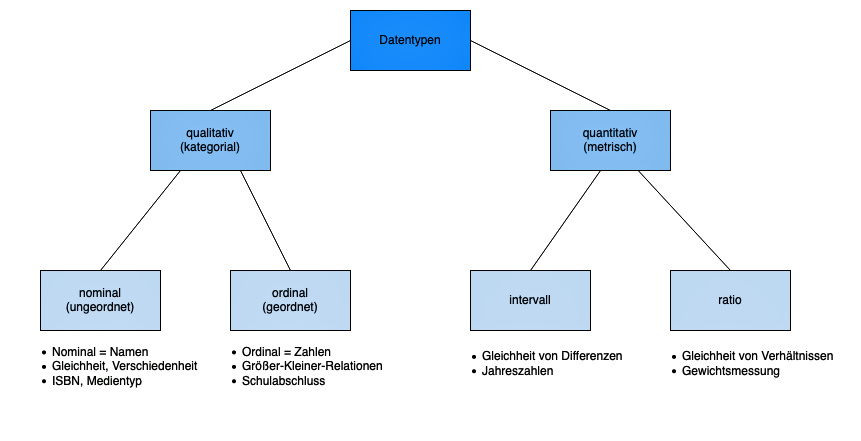
\includegraphics[width=12cm]{datatypes}
        \caption{Statistische Datentypen mit Aussagegehalten und Beispielen}
        \label{fig:data types}
\end{figure}


%Nominale Datentypen können auch Ziffern beinhalten. 
Unterschieden werden die Merkmale ferner nach diskret und stetig.
Ein diskretes Merkmal kann auf der Basis der natürlichen Zahlen abzählbar viele Merkmalsausprägungen annehmen.
So ist zum Beispiel die Größe des Medienbestandes einer Bibliothek ein diskretes Merkmal, da es keine halben oder viertel Medien gibt.
Im Gegensatz dazu können die Merkmalsausprägungen eines stetigen Merkmals jeden beliebigen Wert annehmen. So ist zum Beispiel die Raumtemperatur ein stetiges Merkmal.
Qualitative Merkmale können nur diskret sein, während quantitative Merkmale sowohl diskret als auch stetig sein können \cite[vgl.][102 f.]{kirk_data_2019}. 
Für kategoriale Merkmale eignen sich Balken- und Kreisdiagramme eher als Liniendiagramme, da kategoriale Daten nur diskret sein können.
%Quelle

Der Einsatz von Datenvisualisierungen wird außerdem bestimmt von der Größe der Datenmenge.
Die Darstellung einer großen Datenmenge kann zum Beispiel durch die Wahl eines bestimmten Diagrammes überladen wirken. 
So stößt die Darstellung einer Datenmenge mit vielen Kategorien durch Balken- und Kreisdiagramme 
in der Übersichtlichkeit an Grenzen und kann den Wert der zu erzielenden Aussage verwischen \cite[Vgl.][5 ff.]{few_show_2012}. 

Daten können softwareseitig mit Tabellenkalkulationsprogrammen visualisiert werden.
In Data-Science-Projekten können außerdem verschiedene Frameworks zum Einsatz kommen. Populär sind die Bibliotheken Matplotlib, Seaborn, Plotly für 
die Programmiersprache Python. Für die Programmiersprache R gibt es ebenfalls vielfältige Möglichkeiten der Visualisierung mit
ggplot. Einen Überblick zeigt die Webseite \textquote{The Chart maker}\cite{witherley_chartmaker_2020}.
Eine mächtige und verbreitete JavaScript-Bibliothek zur Datenvisualisierung ist D3.js.
%Interaktivität


%Die dargestellten Daten kommen aus allen Bereichen des Lebens. 
Daten entstehen in wissenschaftlichen Experimenten, aus statistischen Erhebungen wie 
dem Census, auf Kassenzetteln, in Smartphones, in Unternehmen oder in Einrichtungen wie Bibliotheken. 
In Unternehmen werden Datenvisualisierungen eingesetzt, um auf der Managementebene die operative Planung und Entscheidungsfindung zu unterstützen.
Dabei ist Datenvisualisierung ein Bestandteil eines ganzheitlichen Prozess, der unter dem Begriff \acrfull{BI} fungiert. 
%Dieser scheint mittlerweile auch im Bibliothekswesen angekommen zu sein.


%DV für Teile der Daten -> Dateln liegen überall im Unternehmen verstreut in einzelnen Abteilungen
%Teilweise ausgewertet -schwierig für Berichtswesen gegenüber Stakeholdern
%Lsg. wäre eine ganzheitliche IT-Lösung. Diesen Ansatz fährt BI
%Die Präsentation der Daten füe wen ... umschließt Interaktivität -> statischen Bildern hinzu interaktiven \dots
%audience -> stakheoldern -> Berichtswesen oder BI
%zu welchen Zweck -> ...was die Daten beinhalten welche Indikatoren
%Datenvisualisierungen lassen sich bündeln 
%Präsentation den Stakeholdern, um datengetrieben Managemententscheidungen zu erleichtern
%bieten sich BI
%Neuere Entwicklung gehen hinzum Dashboard  - einer Darstellung der wesentlichen Informationen komprimiert \dots
%Dashboards können  als Teil von Business-Intelligence-Systemen verstanden werden.


\section{Business-Intelligence-Systeme}
\acrfull{BI}\footnote{Synonym wird auch manchmal der Begriff Analytische Informationssysteme oder Business-Intelligence-Systeme gebraucht}
bezeichnet allgemein Konzepte und Methoden zur Entscheidungsfindung, die auf
erfassten Informationen beruhen. 
%Aus technischer Sicht umfasst \textit{\acrshort{BI}} unter anderem die Komponenten der Datenhaltung,der  Datenintegration, des Reportings, die \acrfull{OLAP} und Data Mining.
\textit{\acrshort{BI}-Systeme} gehören zu den Management-Support-Systemen, die seit den 1960er Jahren in Unternehmen im Einsatz sind \cite[vgl.][83]{gronwald_integrierte_2020}.

Populär wurde der Begriff \textit{\acrshort{BI}} in den 1990er Jahren. Die Verbreitung des Begriffs fiel zusammen mit der 
Entwicklung einheitlich strukturierter und dauerhaft verfügbarer Datenbanken in Unternehmen, sogenannten Data Warehouses (DWH). 
Grund für diese Entwicklung waren die immer neuen Informationsbedürfnisse auf Managementebene, die schnell befriedigt werden sollten.
%\cite[vgl.][268 f.]{abts_grundkurs_2017}.
Die Einrichtung dieser Datenbanken zielt ab auf eine umfassende Informationsversorgung durch Verdichtung der Unternehmensdaten 
%auf unterschiedlichen Schichten mit detaillierten Kennzahlen. 
%Der Zugriff auf diese Informationen soll jederzeit erfolgen 
\cite[vgl.][268 ff.]{abts_grundkurs_2017}. 

\textit{\acrshort{BI}} beschreibt einen integrierten, unternehmensspezifischen,
IT-basierten Gesamtansatz zur Unterstützung betrieblicher Entscheidungen \cite[vgl.][270]{abts_grundkurs_2017}. 
Ein Hauptmerkmal der \textit{\acrshort{BI}} ist nach \Citeauthor{linden_geschaftsmodellbasierte_2016} die Entscheidungsunterstützung der Managementebene
\cite[vgl.][111]{linden_geschaftsmodellbasierte_2016}. Die Abgrenzung zu operativen
Anwendungssystemen wie \acrfull{OLTP}-Systemen ist laut \citeauthor{abts_grundkurs_2017} ein weiteres wichtiges Merkmal der \textit{\acrshort{BI}}-Systeme \cite[vgl.][267]{abts_grundkurs_2017}. 

Die wesentlichen Schichten eines \textit{\acrshort{BI}-Systems} umfassen die Bereiche der internen und externen Datenlieferanten, den Komplex der Datenintegration und -aufbereitung, 
das Gebiet der Datenspeicherung - und bereitstellung im \textit{\acrlong{DWH}} und den Zweig der Datenanalyse und -präsentation\cites[vgl.][126 ff.]{linden_geschaftsmodellbasierte_2016}[vgl.][8]{kemper_business_2010}. 

Die Schichten der \textit{\acrshort{BI}-Systeme} können in einem Referenzarchitekturmodell abgebildet werden. 
%Dieses Modell kann alle technischen Komponenten umfassen, die von der eigentlichen konkreten Implementierung abstrahiert werden müssen. 
Die Referenzarchitektur kann auch die Datenflüsse zwischen den verteilten Systemeinheiten und Komponenten erfassen \cite[vgl.][126 ff.]{linden_geschaftsmodellbasierte_2016}.
Eine schematische Darstellung in Form eines solchen Referenzarchitekturmodell zeigt die \autoref{fig:bis}.
%In der Fachliteratur wird das Modell oft mit drei Ebenen beschrieben\cites[vgl.][126 ff.]{linden_geschaftsmodellbasierte_2016}[vgl.][8]{kemper_business_2010}.

\begin{figure}[h]
    \centering
        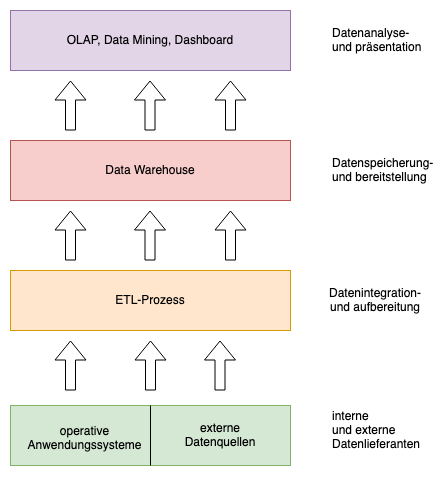
\includegraphics[width=12cm, height=10cm]{bis}
        \caption{Schichten eines Business-Intelligence-Systems}
        \label{fig:bis}
\end{figure}

%Die Ebenen umfassen die Ebene der Datenquellen und Datenerfassung, die Ebene der Datenbereitstellung und Speicherung sowie die Ebene der Datenanalyse und -präsentation.
Von den internen und externen Datenlieferanten werden die Daten im Bereich der Datenintegration und -aufbereitung mithilfe von \textit{\acrshort{ETL}-Prozessen} bearbeitet. 
%Der letzte genannte Bereich wird auch als Staging Area bezeichnet.
In einem ersten Schritt werden die Daten aus den \textit{\acrshort{OLTP}-Systemen} oder aus anderen Datenquellen extrahiert. 
Der anschließende Transformationsprozess wandelt die Daten in ein homogenes Format um. Dabei handelt es sich um einen vierstufigen Prozess. Die Daten werden mit Hilfe 
zum Teil automatischer Verfahren bereinigt, harmonisiert, verdichtet (aggregiert) und angereichert.
Bereinigt werden die Daten unter anderem von syntaktischen und semantischen Mängeln. Unterschiedliche Codierungen der Daten werden durch die Harmonisierung 
beseitigt. Des Weiteren werden die Daten verdichtet, das heißt es werden Summationen von den Daten auf verschiedenen Ebenen durchgeführt und gespeichert. 
Die Berechnung und Speicherung wichtiger Kennzahlen geschieht durch das Verfahren der Anreicherung \cites[vgl.][86]{gronwald_integrierte_2020}[vgl.][277 f.]{abts_grundkurs_2017}.
Schließlich werden die Daten in einem Ladeprozess in das \textit{\acrlong{DWH}} geladen \cite[vgl.][129 ff.]{linden_geschaftsmodellbasierte_2016}. 

Die Datenspeicherung und -bereitstellung erfolgt im \textit{\acrshort{DWH}}. Dieser Bereich ist nach \citeauthor{linden_geschaftsmodellbasierte_2016} zentral für die 
\textit{\acrshort{BI}-Referenzarchitektur}\cite[vgl.][135]{linden_geschaftsmodellbasierte_2016}. Ein \textit{\acrlong{DWH}} ist ein logisch zentralisiertes Datenhaltungssystem. Dieses ist physisch 
von den operativen Anwendungssystemen getrennt und stellt eine harmonisierte Datenbasis für betriebswirtschaftliche Analysen bereit \cite[vgl.][135]{mucksch_data_2000}.\footnote{Alternativen zum Data Warehouse wären verschiedene Data Marts, 
die kleinere Datenspeichereinheiten darstellen und sich inhaltlich an späteren Abfrage- und Auswertungszwecken orientieren.} 
Ein \acrlong{DWH} zeichnet sich durch die vier Merkmale themenorientiert, zeitorientiert, integriert und nicht-volatil aus \cites[vgl.][29 f.]{inmon_building_nodate_2005}[vgl.][271 f.]{abts_grundkurs_2017}[vgl.][136 f. ]{linden_geschaftsmodellbasierte_2016}. Die Speicherung der Daten erfolgt nach Themenschwerpunkten und
orientiert sich am Informationsbedarf des Unternehmens. Die zeitorientierte Speicherung der Daten ermöglicht Zeitreihenanalysen auf historischen Daten. 
Für die Schaffung einer homogenen Datenbasis integriert das \textit{\acrshort{DWH}} die Daten aus heterogenen Datenquellen \cite[vgl.][136]{linden_geschaftsmodellbasierte_2016}.

Die Datenintegration in das \textit{\acrlong{DWH}} kann auf Grundlage  multidimensionaler Datenmodelle wie sogenannten Datenwürfeln erfolgen. 
%Ein \textit{\acrshort{DWH}} kann nach einem Datenwürfel (data cube) konzeptuell modelliert.
Multidimensionale Datenwürfel können n-Dimensionen haben. Sie bestehen mit Fakten und Dimensionen aus zwei Elementen. 
Fakten sind Kennzahlen, die in den Zellen des multidimensionalen Würfels enthalten sind.
Dimensionen sind Entitäten, die um einen Fakt angeordnet sind. Die Dimensionen spannen die Kanten des multidimensionalen Datenwürfels auf.
%Die Anzahl der Kanten entspricht der Dimensionalität eines Würfels.
Die Betrachtung der Kennzahlen ist so in einem multidimensionalen Datenmodell anhand verschiedener Dimensionen möglich 
\cites[vgl.][13 ff., 21 f.]{farkisch_data-warehouse-systeme_2011}[vgl.][66 f.]{kemper_business_2010}.
%OLAP-Funktionalitäten werden zum Navigieren in den Dimensionen der Datenwürfels genutzt, ebenfalls für
%die Ermittlung aggregierter Kennzahlenwerte. 
%Ebenso sind durch Hierarchien die Unterteilung der Auswertungsebenen realisierbar.
%Die Daten entsprechen den Dimensionen des Würfels. Diese können über die Achsen des Würfels ausgewählt und kombiniert werden. 
%Diese multidimensionale Datenstruktur bietet einen multidimensionalen Blick auf die Daten und erlaubt dadurch Vorberechnungen und einen schnellen Zugriff auf summierte Daten.  
%Die Umsetzung des multidimensionalen Modells kann durch relationale (ROLAP) oder multidimensionale (MOLAP) geschehen.

Ein \textit{\acrlong{DWH}} bietet des Weiteren eine nicht-volatile Speicherung der Daten an. Damit ist sichergestellt, dass auf diesen Daten längerfristige Analysen durchgeführt werden können \cite[vgl.][136]{linden_geschaftsmodellbasierte_2016}.
In die Konzeptionierung eines \textit{\acrlong{DWH}s} sollten deswegen Archivierungskonzepte und zudem Überlegungen zu den Aktualisierungszyklen der Daten für das \textit{\acrshort{DWH}}
miteinfließen. Die Archivierungskonzepte sorgen dafür, dass veraltete Datenbestände gesichert und komprimiert werden.
Die Aktualisierungszyklen legen fest, in welcher periodischen Abfolge die Daten aktualisiert werden, entweder zu Zeitpunkten der Änderungshäufigkeit
der Daten im operativen Anwendungssystem, in periodischen Zeitabständen oder aber auch in Echtzeit \cite[vgl.][137]{linden_geschaftsmodellbasierte_2016}.

Bei der Umsetzung mit Datenbanktechnologien besteht die Möglichkeit, das multidimensionale Modell in einer relationalen Datenbank umzusetzen.  
%beziehungsweise eine eigene Tabelle für Fakt und jede Dimension anzulegen. 
Realisiert werden kann dies mit einer logischen Datenmodellierung durch ein Star- oder Snowflake-Schema\cite[vgl.][177 f.]{linden_geschaftsmodellbasierte_2016}.



%Dabei ist zu beachten, dass es ein Archivierungskonzept geben muss und darüber hinaus sind Aktualiaierungszyklen 
%des \acrshort{DWH} festzulegen. Nach Änderungshäufigkeit der Daten im Vorsystem, einem Zeitfenster oder in Echtzeit (138 ff.)
%Alternativen zum Data Warehouse wären verschiedene Data Marts, die kleinere Datenspeichereinheiten darstellen 
%und die sich inhaltlich an späteren Abfrage- und Auswertungszwecken orientieren. Andere Idee wäre noch ein Data Lake.

Die letzte Schicht eines \textit{\acrshort{BI}-Systems} umfasst die Datenanalyse und -präsentation. Die Datenanalyse kann verschiedene Auswertungskonzepte aufweisen.
Die Auswertungskonzepte bieten spezifische Funktionen für Analysen an. Im Rahmen herkömmlicher \textit{\acrshort{BI}-Systeme} werden \acrfull{OLAP}-Verfahren angewendet. 
\textit{\acrshort{OLAP}} ist eine Anfragetechnik für die Analyse multidimensionaler oder relationaler Daten. Diese Technik erlaubt es, Daten mit \textit{\acrshort{OLAP}}-Funktionen 
wie Drill-Down, Roll-up, Slice oder Dice auf verschiedenen Stufen mit unterschiedlichen Sichtweisen darzustellen. So ist eine Verfeinerung der Analyseergebnissen (Drill-Down) und 
deren Aggregation möglich. Darüber hinaus können Teilmengen durch Slicing und Dicing gebildet werden \cite[vgl.][283 f.]{abts_grundkurs_2017}. 
Durch OLAP-Anwendungen können die multidimensionalen Datenstrukturen interaktiv ausgewertet werden.
%Durch die Bereitstellung multidimensionaler Daten in einem Datenwürfel im  \acrlong{DWH}, werden direkt \textit{\acrshort{OLAP}}-Funktionen wie drill-down, roll-up, slice oder dice ermöglicht. 
%Drill-Down erlaubt zum Beispiel einen detaillierteren Blick auf die Daten, während sich mit der roll-up-Operation sich Daten auf einer höheren Hierarchiestufe betrachten lassen.

Ein anderes Verfahren ist Data Mining. Data Mining benutzt verschiedene statistische und mathematische Verfahren, um Muster und Trends in vor allem
großen Datenmengen zu entdecken. Klassische Data-Mining-Aufgaben sind Ausreißer-Erkennung, Klassifikation, sowie die Cluster- , Assoziations- und Regressionsanalysen \cite[vgl.][15 ff.]{han_data_2012}.
Data Mining wird entweder synonym gesetzt mit dem Prozess der \acrfull{KDD} oder als Teilphase dieses Prozesses beschrieben
\cites[vgl.][6]{han_data_2012}[vgl.][142 f.]{linden_geschaftsmodellbasierte_2016}.
Data-Mining-Verfahren können als zusätzliche Auswertungsverfahren zu \textit{\acrshort{OLAP}}-Verfahren hinzutreten.

Die Datenpräsentation umfasst die strukturierte und visuelle Darstellung der zuvor angewendeten Analyseverfahren.
% in hochaggregierter, verdichteter, quantitativer wie qualitativer Information. Diese Information sind Dies kann geschehen durch  \textit{\acrshort{BI}-Portale} oder durch Dashboards.(154)
Die Präsentation der Daten kann durch Reporting oder Dashboards erfolgen. Über Reporting-Tools können Standardberichte generiert werden. 
Diese statischen Berichte können nicht verändert werden. Für die Darstellung der Daten in diesen Berichten werden
Tabellen, Listen und Diagramme verwendet. Der Bericht kann bereitgestellt werden in PDF-Format \cite[vgl.][114]{bange_werkzeuge_2016}.


Im Gegensatz dazu ermöglichen Dashboards einen interaktiven Zugang über eine Benutzungsoberfläche zu den relevanten Informationen.
Nach \Citeauthor{few_information_2006} ist ein Dashboard ein \textquote{ ... visual display of the most important 
information needed to achieve one or more objectives; consolidated and arranged on a single screen so the
information can be monitored at a glance.} \cite[26]{few_information_2006} Dashboards werden im unternehmerischen Rahmen auch Performance Dashboards genannt \cite[vgl.][154]{linden_geschaftsmodellbasierte_2016}.
Diese werden verschieden klassifiziert. Sie lassen sich nach Reichweite und Zweck einteilen. Es gibt operative, taktische (analytische) oder strategische Dashboards. 


Operative Dashboards überwachen und kontrollieren gegenwärtige Geschäftsprozesse. Durch die hohe Aktualisierungsfrequenz der Daten kann schnell in 
die betrieblichen Prozesse steuernd eingegriffen werden \cites[vgl.][11 f.]{eckerson_performance_2011}[vgl.][30 f.]{few_information_2006}.


Taktische oder analytische Dashboards konzentrieren sich auf verschiedene Bereiche des Unternehmens 
und bieten Möglichkeiten einer anforderungsgerechten und lösungsorientierten Analyse durch eine Bewertung der Daten auf mehreren Detailebenen. 


Strategische Dashboards repräsentieren hochaggregierte Kennzahlen, die langfristige Ziele und deren Erreichungsgrade visualisieren. 
Sie werden zur Kommunikation und Kollaboration auf oberster Managementebene genutzt \cite[vgl.][155 f.]{linden_geschaftsmodellbasierte_2016}. 


Die Grenzen zwischen den Dashboards bezüglich Reichweite und Zweck sind aber nicht trennscharf. 
So kann es Überlappungen zwischen strategischen, taktischen und operativen Dashboards geben \cite[vgl.][121]{eckerson_performance_2011}.


Neuere Entwicklungen in den \textit{\acrshort{BI}-Systemen} führen weg von der strikten Trennung zwischen \acrshort{OLTP} und und \acrshort{OLAP} und zur Auflösung der \textit{\acrshort{DWH}}. 
Anstelle derer treten Data Lakes. Data Lakes speichern im Gegensatz zu den \acrlong{DWH}s die Rohdaten in strukturierter oder unstrukturierter Form. 
Mitunter wird dabei auf die aufwändigen \textit{\acrshort{ETL}-Prozesse} verzichtet \cite[vgl.][86]{gronwald_integrierte_2020}, und die Daten werden zum Analysezeitpunkt bearbeitet.


%\section{Zusammenfassung}


% Bereitstellung einer interaktiven Nutzung und Navigation der Kennzahlen
% Darstellung hochaggregierter, verdichteter und quantitativer und qualitativer Information
% Klassifizierung von Dashboards
% Performance Dashboard -> Ziel: steuerndes Eingreifen nach Analyse der Ursachen
% -> strategische, taktische oder operative Reichweite -> Zweck: Kommunikation btw. Kollaboration, Analyse und Monitoring



% %Dashboards
% %Bilder BI-Systeme
% %OLAP
% %Data-Mining
% % Data Lake

% Für das zu entstehende System sind die drei Ebenen wichtig. Der ETL-Prozess, Die Datenhaltung und -bereitstellung und die Datenanalyse und - Präsentation.
% % Wichtig ist die Staging Area, da die Daten in heterogenen Daten vorliegen, die Frage der Datenhaltung ist noch nicht geklärt entweder DataLake oder doch eine relationale
% Datenbank. Die Frage der Analyse müsste noch geklärt werden inwieweit ein an OLAP angelehntes Verständnis zielführender wäre oder Data Mining. Für die Präsentation ist ein Dashboard
% geplant, dass monitoriong charakter annehmen soll. Daraus ergeben sich Anforderungen, die im nächsten Kapitel ausformuliert werden. 

% %OLAP
% %Technik, die flexible Analysen auf Datenbestände durchführt. Möglichkeit Unternehmensdaten aus verschiedenen Sichtweisen darzustellen

% %Data Mining
% %technik, die statitische Methoden und Algorithmen auf einen Datenbestand anwendet, um Muster und Zsh. zu erkennen. 

% %Die Entwicklung IT-unsterstützender Systeme fängt in den 1960er Jahren an.
% %\acrfull{DWH}\\
% %In dem Zusammenhang bit BI bedeuted Data Ware House eine themenorientierte, vereinheitlichte, beständige, zeitbezogene
% %Sammlung von Daten zur Unterstützung von Managemententscheidungen\cite[vgl.][271]{abts_grundkurs_2017}
        
% %Data Lake:


% \clearpage
% %%%%%%%%%%%%%%%%%%%%%%%%%%%%%%%%%%%

% BI- Systeme (Data Ware House System) mit ganzheitlichen Ansatz
%     Datenbanken, Datenquellen
%     Datenflüsse zwischen den verteilten Systemeinheiten unf Komponenten
% BI-Referenzarchitektur
% 1. Ebene der Datenquellen- und Datenerfassung
%     Datenextraktionsphase (S. 129 f.)
%         Ausgangspunkt: operative Vorsysteme (Transaktionssysteme) = interne Datenquellen einer Organisation
%         Vereinheitlichung der heterogenen Daten aus verschiedenen Datenquellen und Zusammenführung in einer Datenbank => ETL-Prozess
%         => zur Herstellung einer inhaltlich konsistenten Datenbasis.
%         Festlegung eines Prozess nach Peridodizität oder nach Ereignis => Herausziehen der Daten aus den operativen Vorsystemen       
%     Datentransformationsphase (130 f.)
%         inhaltliche und strukturelle Umwandlung der Daten in ein homogenes Format
%         Staging  Area
%             Filterung => Auswahl, Bereinigung (syntaktische (Sonderzeichen) und semantische Mängel (fehlende Werte) => mögliche Erkennung mit automatisierten Verfahren) und Speicherung der Datenextrakte, 
%         Harmonisierung (132)=>???, 
%         Aggregation
%         Anreicherung
%     Datenladephase (133)
%         Ladeprozess der die Daten in das Core Data Warehouse (= Gesamtbild der Unternehmensaktivitäten) lädt (mit evtl. Umweg über andere vorgelagerte Datenbanken)
        
%   und weiterzuführende betriebswirtschaftliche Analysen ermöglicht
% 2- Ebene der Datenhaltung und Bereitstellung (135 ff.)
%     zentraler Bereich der BI-referenzarchitektur
%     Core Data Warehouse (= Gesamtbild der Unternehmensaktivitäten) => Bereitstellung einer konsistenten Datenbasis
%     logisch zentralisiertes, unternehmensweites datenhaltungssystem, das physisch von den operativen Vorsystemen getrennt, eine harmonisierte Datenbasis darstellt,
%     und weiterzuführende betriebswirtschaftliche Analysen ermöglicht
%     dauerhafte Speicherung der Daten, damit längerfristige Analysen durchgeführt werden können -> Zeitreihenanalysen vor Hintergrund historisierter Datenbestände
%     Archivierungskonzepte müssen vorliegen


%     Es gibt eine Vielzahl kommerzieller Lösungen für den Bibliotheksbereich, die auf Business-Intelligence-Systemen basieren.
%     Zu nennen wären \textit{AlmaAnalytics} für das Next-Generation-Library-System \textit{Alma} von \textit{ExLibris}\footnote{\url{https://www.exlibrisgroup.com/products/alma-library-services-platform/alma-analytics}
    
%     Stand: 26.05.2020}, \textit{BibControl} von \textit{OCLC}\footnote{\url{https://www.oclc.org/de/bibcontrol.html} Stand: 26.05.2020},
%     \textit{CollectionHq} von \textit{Baker \& Taylor}\footnote{\url{https://www.collectionhq.com/} Stand: 26.05.2020} oder \textit{Libinsight} von \textit{SpringShare}\footnote{\url{https://springshare.com/libinsight/} Stand: 26.05.2020}.
%     Darüber hinaus gibt es Business-Intelligence-Applikationen, die von
%     Bibliotheken für Reporting, Datenanalyse und Datenvisualisierung adaptiert werden,
%     wie zum Beispiel \textit{Tableau} von der Firma \textit{Tableau Software} oder
%     \textit{Crystal Reports} von \textit{SAP}.
%     Diese Applikationen sind entweder
%     an bestimmte Bibliothekssysteme zurückgebunden, limitiert in ihren
%     Funktionen\cite{golas_statistische_2018} oder zu generisch.
%     %Überdies wird sowohl von \textit{HeBis} bzw. von der
%     %Lokal-Bibliothekssystembetreuung als auch von der \textit{mpdl} keine Applikation
%     %in dieser Richtung angeboten.
%     %Ebenso ist ungewiss, wann die Ablösung des schon betagten \textit{CBS/LBS} hin zu
%     %einem neuen Next-Generation-Library-System im \textit{HeBis-Verbund} stattfinden wird und ob
%     %es ein Modul zur statistischen Datenerhebung liefern wird.
